\documentclass[12pt]{article}
\usepackage{hyperref}
\usepackage{xcolor}
\usepackage{framed}
\usepackage{listings}
\usepackage{graphicx}
\usepackage{float}
\usepackage{pdfpages}
\usepackage[utf8]{inputenc}
\usepackage[T1]{fontenc}

\usepackage{titlesec}
\newcommand{\sectionbreak}{\clearpage}

\makeatletter
\renewcommand{\@seccntformat}[1]{}
\makeatother

\setlength{\parindent}{0pt}
%\newcommand{\response}[1]{{\leavevmode\color{blue}[#1]}}
\newcommand{\response}[1]{\color{blue}{#1}\color{black}}

\definecolor{mygreen}{rgb}{0,0.6,0}
\definecolor{mygray}{rgb}{0.5,0.5,0.5}
\definecolor{mymauve}{rgb}{0.58,0,0.82}
\definecolor{light-gray}{gray}{0.95}

\lstset{ %
  backgroundcolor=\color{light-gray},   % choose the background color
  basicstyle=\footnotesize,        % size of fonts used for the code
  breaklines=true,                 % automatic line breaking only at whitespace
  captionpos=b,                    % sets the caption-position to bottom
  commentstyle=\color{mygreen},    % comment style
  escapeinside={\%*}{*)},          % if you want to add LaTeX within your code
  keywordstyle=\color{blue},       % keyword style
  stringstyle=\color{mymauve},     % string literal style
}

\begin{document}

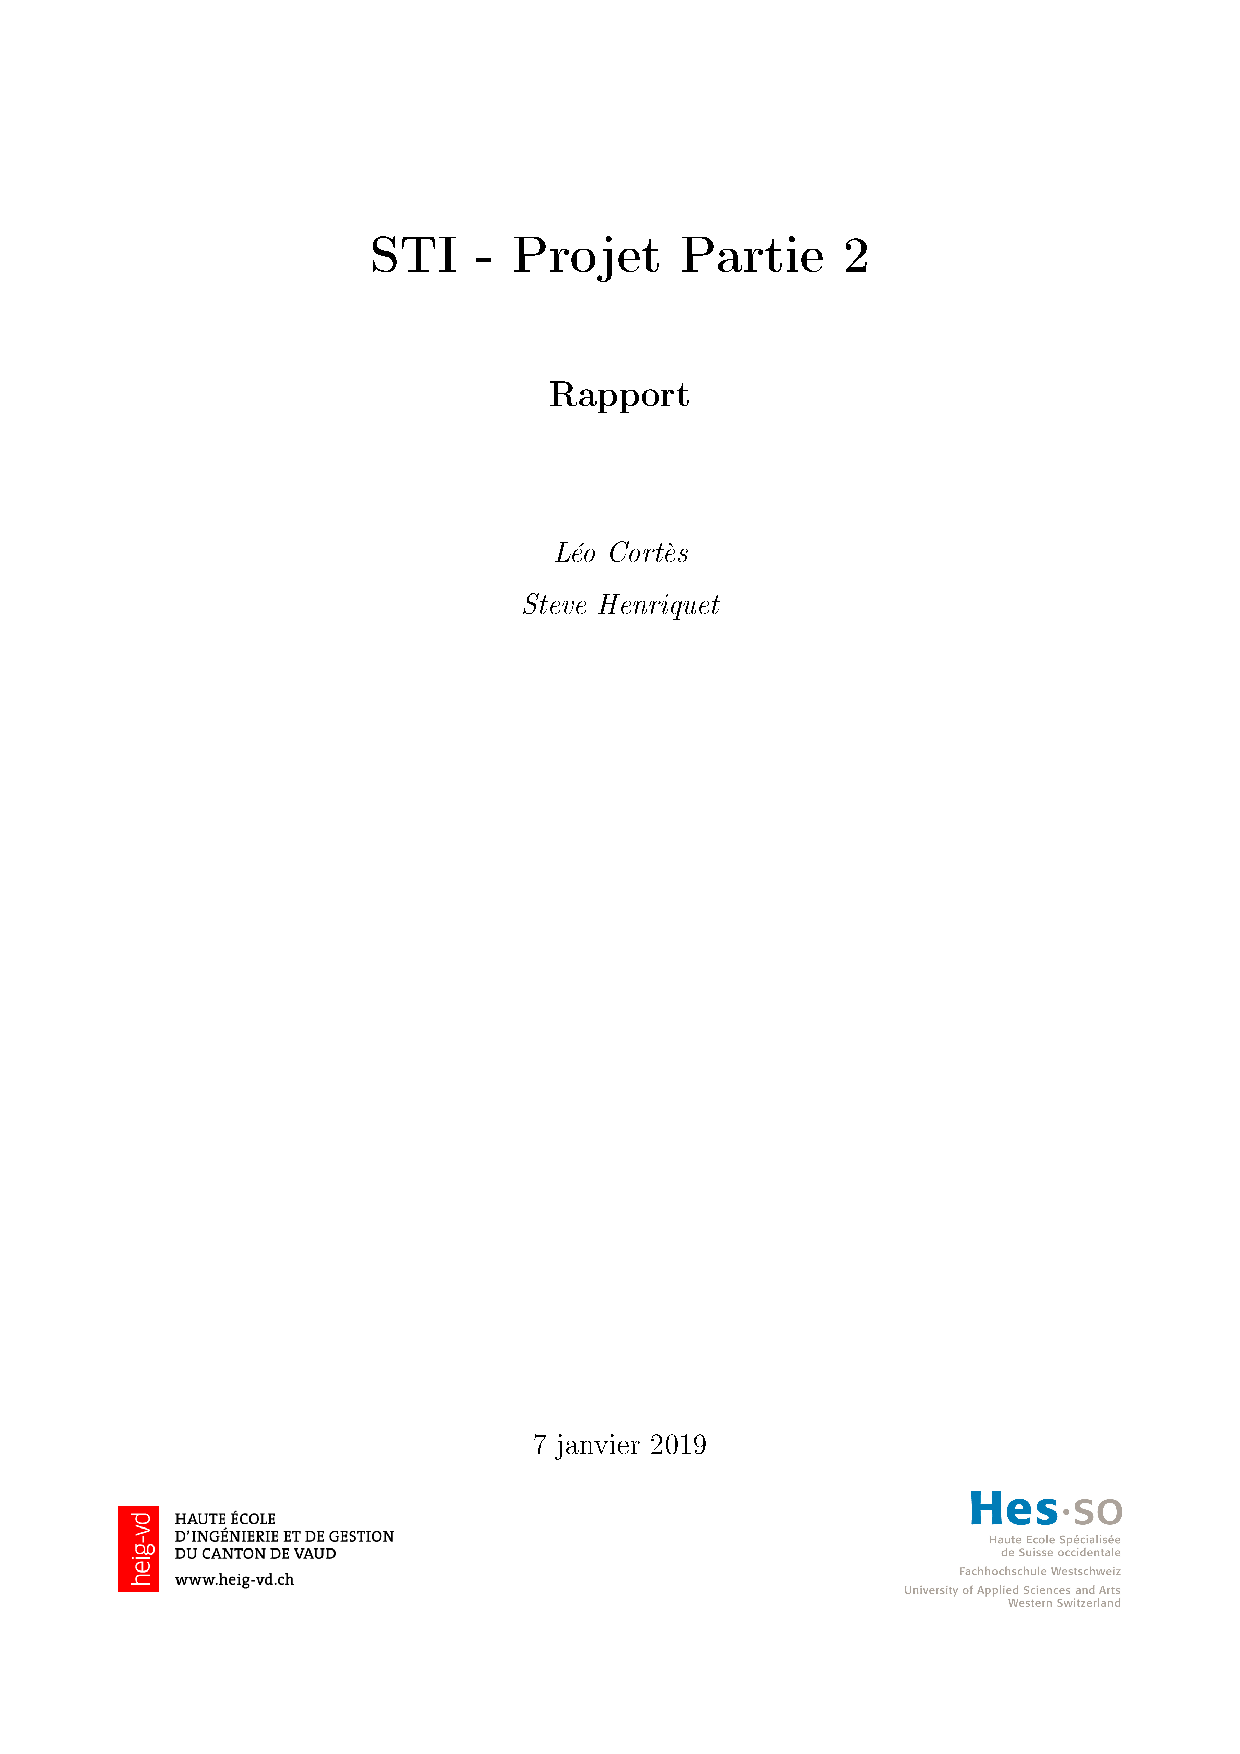
\includepdf{titre/titre.pdf}

\tableofcontents

\newpage
\section{Introduction}

\section{Analyse de menaces}
\subsection{Agents menaçants}
En principe, notre application devraient être accessibles depuis n'importe qui sur Internet. Les agents menaçants peuvent donc être n'importe qui. Notre application n'est pas révolutionnaire et bien moins efficace que la concurrence. Des attaquants concurrents seraient donc peu probables. Les principaux agents menaçants seraient surtout nous (les élèves du cours STI) ou n'importe quelle personne souhaitant s'amuser.

\subsection{Vecteurs d'attaque}
Tout se passe sur le web. Les utilisateurs peuvent (et doivent) manipuler des entrées pour envoyer des messages ou mettre à jour leurs profils. Des entrées malveillantes pourraient exploiter des vulnérabilités au sein de notre application.

\subsection{Faiblesses de sécurité}
Comme nous avons accès au code ne notre application, nous avons une idée des vulnérabilités que nous pouvons y trouver. Dans un premier temps, les entrées utilisateur ne sont pas assainies et sont envoyées telle quelle. Cela laisse place à de nombreuses failles comme des injections SQL ou des XSS.

De plus, les accès à la DB n'utilisent pas de query pré-préparées. Cela pourrait donc donner lieu à des injections SQL supplémentaires.

L'application utilise du HTTP simple et aucun chiffrement. Des données pourraient donc être sniffées et si une fuite de données à lieu, toutes les données pourraient être accessibles en clair.

\subsection{Contrôle de sécurité}
Les accès sont, en principe, vérifiés. Un utilisateurs ne peut accéder qu'aux mails qu'il a envoyé ou reçu et pas ceux d'autres utilisateurs. Les accès administrateurs sont réservés aux administrateurs. Finalement, il n'est pas possible d'accéder à des fichiers stockés sur le serveur. Si un utilisateur essaie d'accéder à une page non prévue, il sera redirigé.

\subsection{Impacts techniques}
Si des messages sont accédés par des personnes non autorisées, cela peut entraîner une perte de confidentialité.

Un accès non autorisé pourrait donner le droit à un attaquant de modifier, voire supprimer de l'information. Une perte d'intégrité peut donc en découler.

\subsection{Impacts business}
L'impact business serait faible. En effet, notre application n'est pas conçue dans un but lucratif et ne sera probablement pas maintenue par la suite. Si une telle application était mise en production dans le but d'offrir un service sérieux, cela pourrait être problématique car des clients pourraient stocker des informations personnelles voire confidentielles  dans leurs messages. Une fuite de données ou des vulnérabilité pourrait entraîner une perte de confiance complète des utilisateurs.

\section{Vulnérabilités et corrections}
\subsection{XSS}
\subsubsection{Exploitation}
Le programme est vulnérable aux attaques XSS. Les balises HTML sont correctement inteprétée, ainsi que les balises de script. C'est problématique car un attaquand pourrait envoyer un message malicieux à un administrateur. Lorsque l'admin se connecte, le script pourrait récupérer ses cookies et l'attaquant pourrait les rejouer et devenir donc administrateur.

Voici le message envoyé par un attaquant quelconque : 
\begin{figure}[H]
\centering
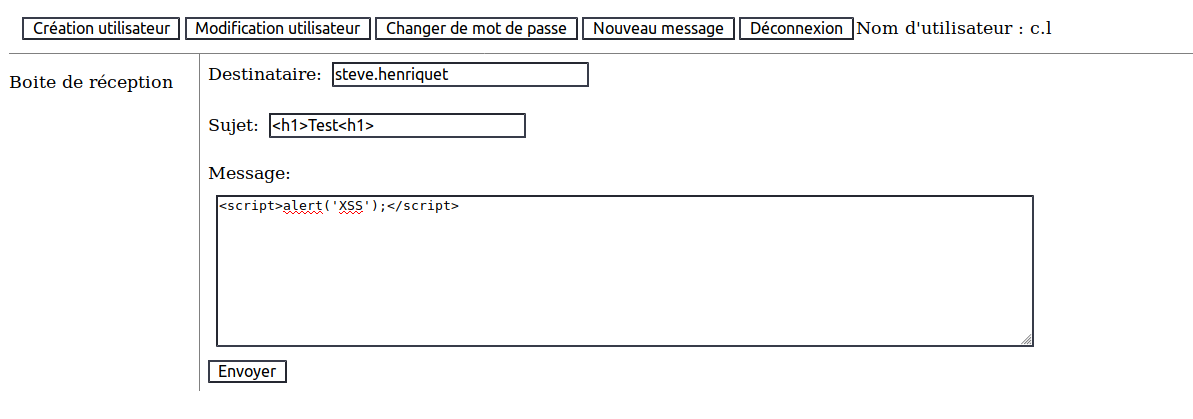
\includegraphics[width=\linewidth]{images/xssAttack.png}
\caption{Message malicieux}
\end{figure}

Voici le résultat dans la boîte de réception de la victime.
\begin{figure}[H]
\centering
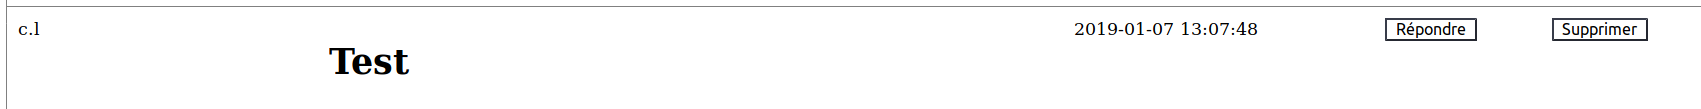
\includegraphics[width=\linewidth]{images/xssRecep.png}
\caption{Boîte de réception}
\end{figure}

Lorsque la victime l'ouvre, voici le script est correctement exécuté.
\begin{figure}[H]
\centering
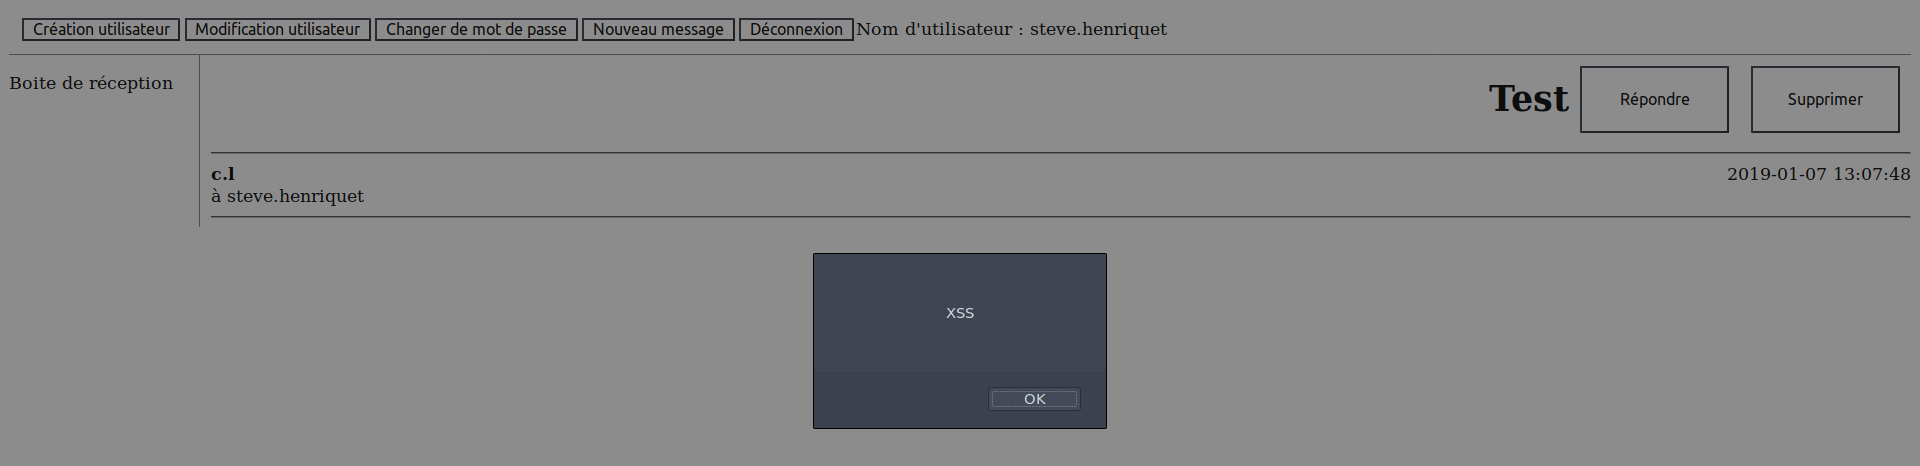
\includegraphics[width=\linewidth]{images/xssOpen.png}
\caption{Exécution XSS}
\end{figure}

\subsubsection{Correction}
Les entrées ont du être "sanitisées". Nous avons utilisé le filtre \textit{FILTER\_SANITIZE\_STRING} dans les divers inputs accessibles.
\begin{figure}[H]
\centering
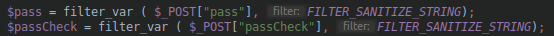
\includegraphics[width=\linewidth]{images/sanitize.png}
\caption{Exemple d'assainisation}
\end{figure}

\subsection{Injection SQL}
\subsubsection{Exploitation}
D'après l'outil \textit{SQLMap}, on peut déjà sortir quelques informations depuis la page de login, dont les tables de notre DB. 

\begin{figure}[H]
\centering
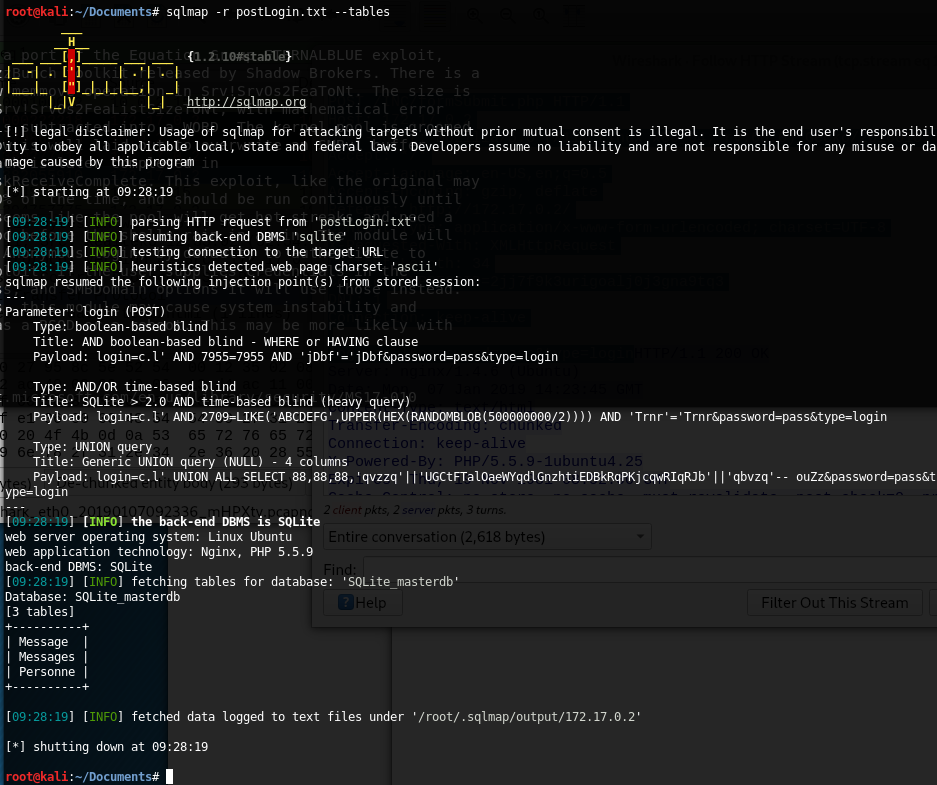
\includegraphics[width=\linewidth]{images/sqli.png}
\caption{Résultat de \textit{SQLMap} sur la page de login}
\end{figure}

\subsubsection{Correction}
Tout comme pour les failles XSS, les entrées ont du être assainies. De plus, les query simples utilisées dans le code PHP ont été passées en prepared statements.

TODO INSERT CODE SCREENSHOTS

\subsection{Mauvaise destruction des session}
\subsection{Exploit}
Les sessions sont mal détruites. Potentiellement, après le login d'un admin, un utilisateur pourrait se retrouver à avoir accès à des informations réservées aux administrateurs.
\begin{figure}[H]
\centering
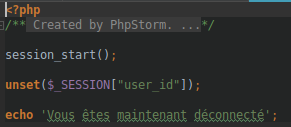
\includegraphics[width=\linewidth]{images/unset.png}
\caption{Mauvaise destruction de la session}
\end{figure}


\subsection{Correction}


\subsection{Accès au page sans login}
\subsubsection{Exploitation}
Envoie de mail par exemple.
\begin{figure}[H]
\centering
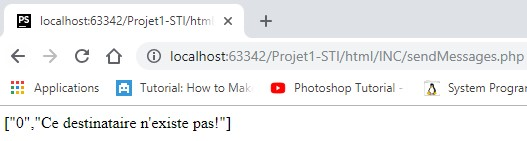
\includegraphics{images/withoutLogin.jpg}
\caption{Accès à la page}
\end{figure}
\begin{figure}[H]
\centering
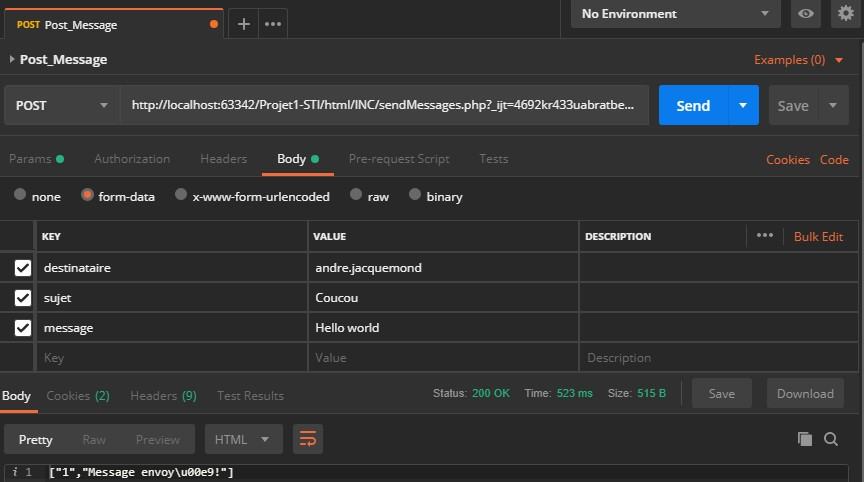
\includegraphics[width=\linewidth]{images/postmanSendMessage.jpg}
\caption{Requête Post réussi}
\end{figure}
\begin{figure}[H]
\centering
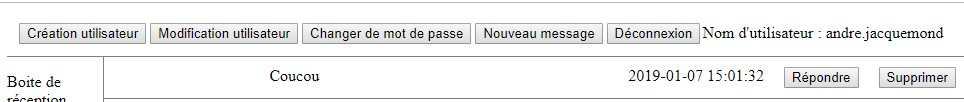
\includegraphics[width=\linewidth]{images/postmanSendMessageSuccess.jpg}
\caption{Message reçu}
\end{figure}

\subsubsection{Correction}
Vérification de l'existante de la variable de session \textit{\$\_SESSION["user\_id"]}.
\begin{figure}[H]
\centering
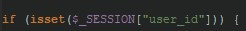
\includegraphics[width=\linewidth]{images/protectionPage.jpg}
\caption{Protection à ajouter aux différentes pages}
\end{figure}
L'ajout de cette vérification s'effectue sur tous les fichiers à l'execption de index.php, login.php et des fichiers effectuant déjà la vérification par rapport au fait d'être administrateur


\subsection{Problèmes non résolvables}
\begin{itemize}
\item PHP 5.6
\item Gestion des cookies de session
\end{itemize}

\end{document}